\chapter{Results}
In this chapter results of both simulations are compared and presented as graphs of velocity components and turbulent quantities along lines $x=0.2$ (figures \ref{fig::ux2} - \ref{fig::nut2}) and $x=0.2$ (figures \ref{fig::ux15} - \ref{fig::nut15}) .
The first sampling line is located \SI{0,1}{\meter} past the inlet to the trimmed domain (and \SI{0,2}{\meter} from flat plate starting point, see figure \ref{fig::flatplate}). The second one is located near the outlet of both domains.

\begin{figure}[h]
\centering
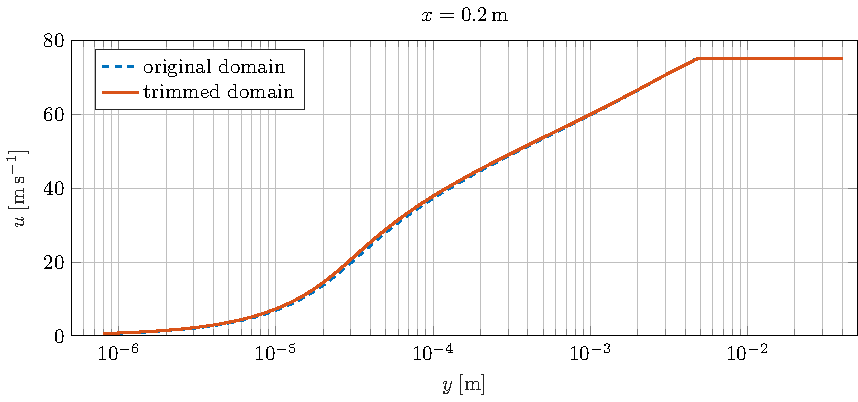
\includegraphics[width=13.5cm]{Results/ux2.pdf}
\caption{Graph of $x$ component of velocity field along the $x=0.2$ line from both original domain and the trimmed one.}
\label{fig::ux2}
\end{figure}

\begin{figure}[h]
\centering
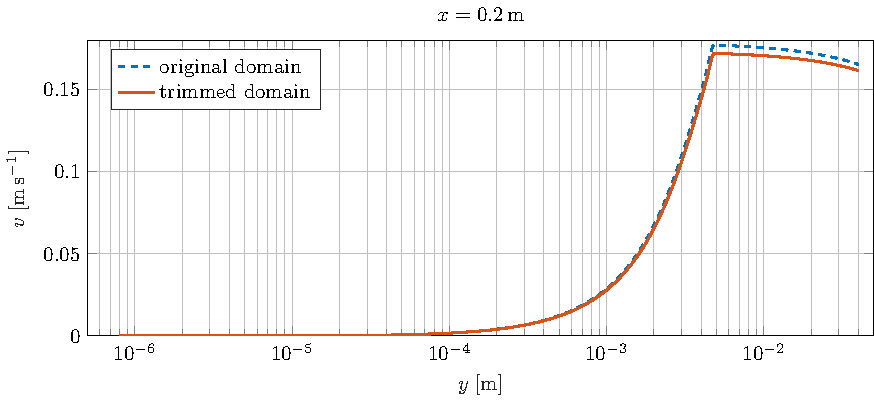
\includegraphics[width=13.5cm]{Results/uy2.pdf}
\caption{Graph of $y$ component of velocity field along the $x=0.2$ line from both original domain and the trimmed one.}
\label{fig::uy2}
\end{figure}

\begin{figure}
\centering
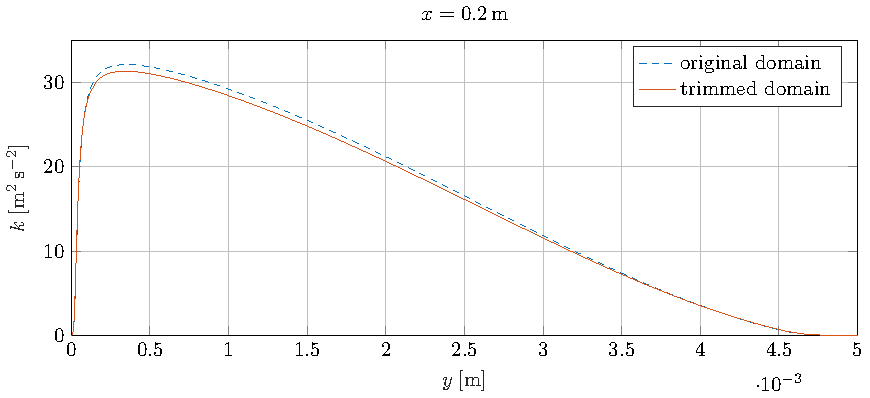
\includegraphics[width=14cm]{Results/k2.pdf}
\caption{Graph of turbulent kinetic energy field along the $x=0.2$ line from both original domain and the trimmed one.}
\label{fig::k2}
\end{figure}

\begin{figure}
\centering
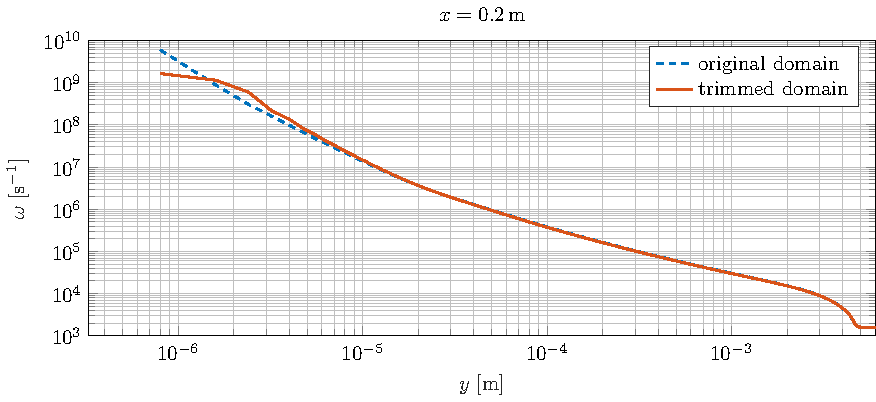
\includegraphics[width=14cm]{Results/omega2.pdf}
\caption{Graph of specific dissipation rate field along the $x=0.2$ line from both original domain and the trimmed one.}
\label{fig::omega2}
\end{figure}

\begin{figure}
\centering
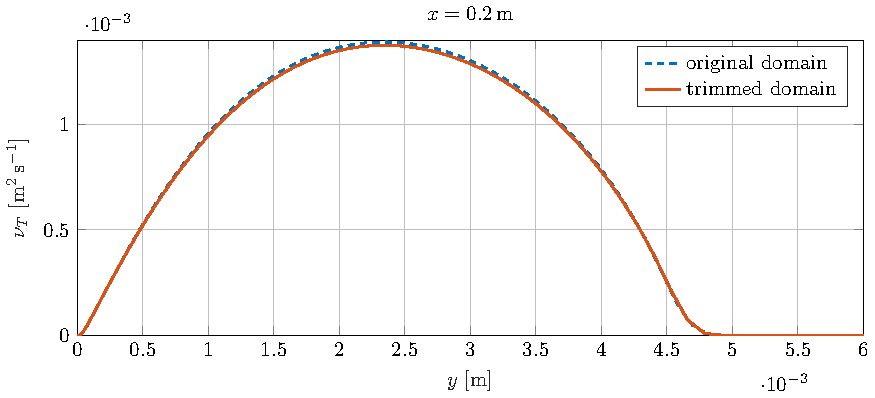
\includegraphics[width=14cm]{Results/nut2.pdf}
\caption{Graph of turbulent viscosity field along the $x=0.2$ line from both original domain and the trimmed one.}
\label{fig::nut2}
\end{figure}

\begin{figure}
\centering
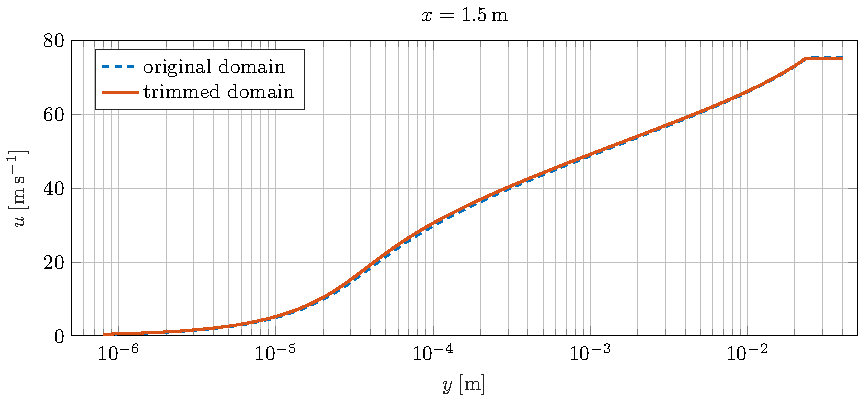
\includegraphics[width=14cm]{Results/ux15.pdf}
\caption{Graph of $x$ component of velocity field along the $x=1.5$ line from both original domain and the trimmed one.}
\label{fig::ux15}
\end{figure}

\begin{figure}
\centering
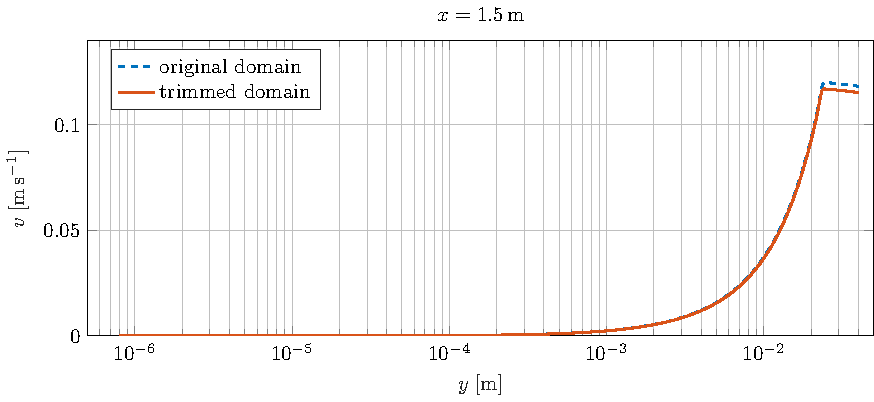
\includegraphics[width=14cm]{Results/uy15.pdf}
\caption{Graph of $y$ component of velocity field along the $x=1.5$ line from both original domain and the trimmed one.}
\label{fig::uy15}
\end{figure}

\begin{figure}
\centering
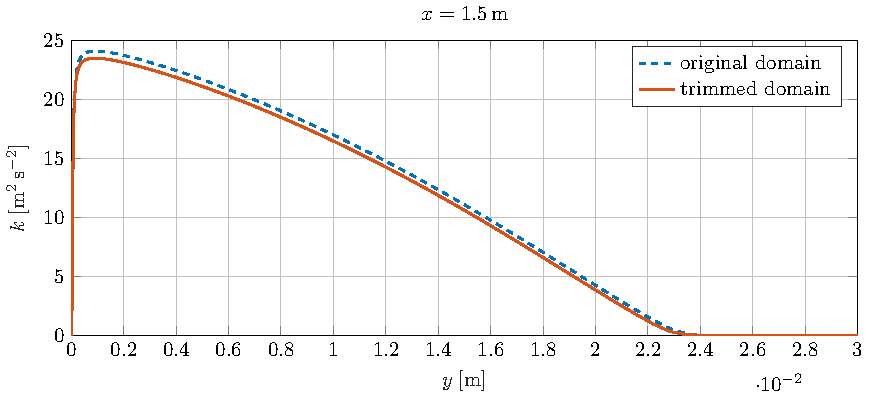
\includegraphics[width=14cm]{Results/k15.pdf}
\caption{Graph of turbulent kinetic energy field along the $x=1.5$ line from both original domain and the trimmed one.}
\label{fig::k15}
\end{figure}

\begin{figure}
\centering
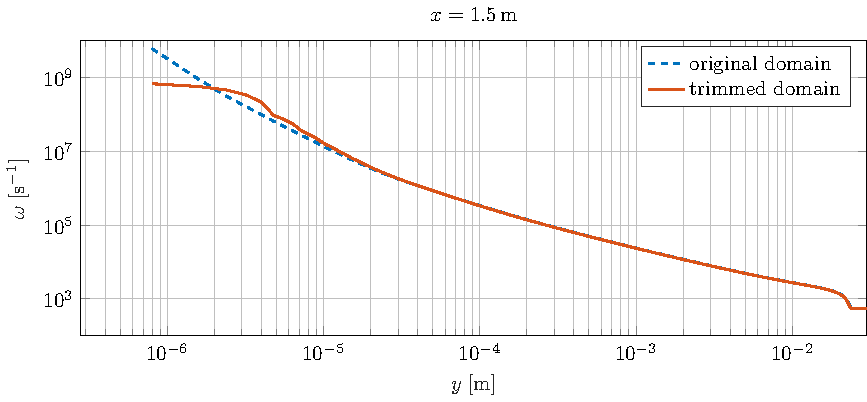
\includegraphics[width=14cm]{Results/omega15.pdf}
\caption{Graph of specific dissipation rate field along the $x=1.5$ line from both original domain and the trimmed one.}
\label{fig::omega15}
\end{figure}

\begin{figure}
\centering
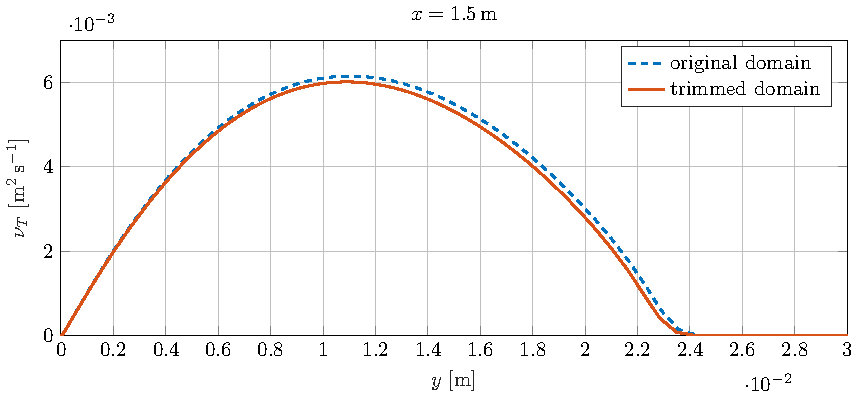
\includegraphics[width=14cm]{Results/nut15.pdf}
\caption{Graph of turbulent viscosity field along the $x=1.5$ line from both original domain and the trimmed one.}
\label{fig::nut15}
\end{figure}